% Chapter 1

\chapter{Thoughts \& ideas} % Main chapter title

\label{sec:ideas} % For referencing the chapter elsewhere, use \ref{Chapter1} 

\section{Sequential Model-Based Optimization (SMBO)}
Current tests are performed using regular Bayesian Optimization (BO) via Gaussian Processes. Resources are available in \url{src/R} (interactive demo code), \url{notebooks} (jupyter notebooks for the same demos) and \url{output/gp} (output plots for different regression scenarios).

\begin{figure}[h]
	\centering
	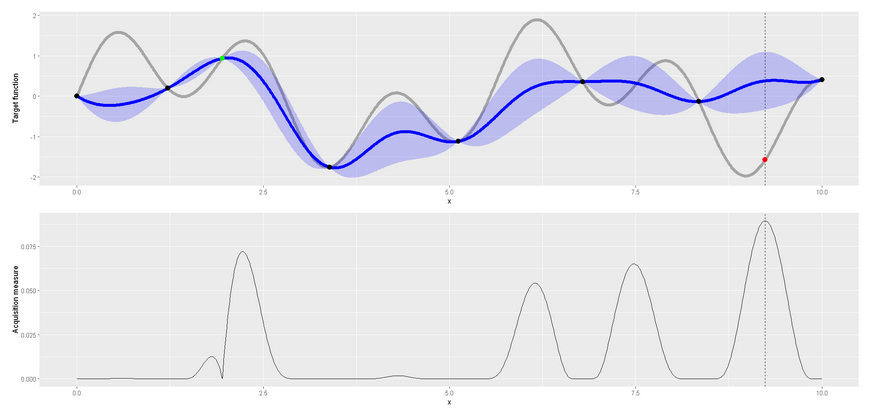
\includegraphics[width=\textwidth]{figures/bo_gp_regression}
	\decoRule
	\caption[Bayesian Optimization]{Bayesian Optimization using a Gaussian process after the eighth observed point. The acquisition function used is the Expected Improvement.}
	\label{fig:bo_gp_regression}
\end{figure}

The error functions that we are trying to optimize, though, are not particularly time-consuming, so other more naive approaches work better by producing good results in a much shorter time (though many more evaluations of the error function). In order to improve this method for these use cases we can focus on different areas.

\subsection{Surrogate model}
Bayesian Optimization uses a surrogate model to approximate the target function and determine the optimal candidates to evaluate for each iteration. The default choice in many cases is a Gaussian Process but other alternatives exist, such as random forests or Tree Parzen Estimators (TPE) [\cite{rasmussen_gaussian_2006}][\cite{bergstra_algorithms_2011}].

\subsection{Kernel selection/composition}
One crucial hyperparameter in the BO method is the kernel. This function determines how the uncertainty over the regression curve is determined and its properties can greatly influence the fit and inference performance of the surrogate model (figure \ref{fig:bo_gp_kernel}). An important step in the optimization procedure will be the selection and/or composition of kernels for the optimization problem [\cite{repicky_automated_nodate}][\cite{duvenaud_automatic_nodate}][\cite{duvenaud_additive_2011}][\cite{duvenaud_structure_2013}].

\begin{figure}[h]
	\centering
	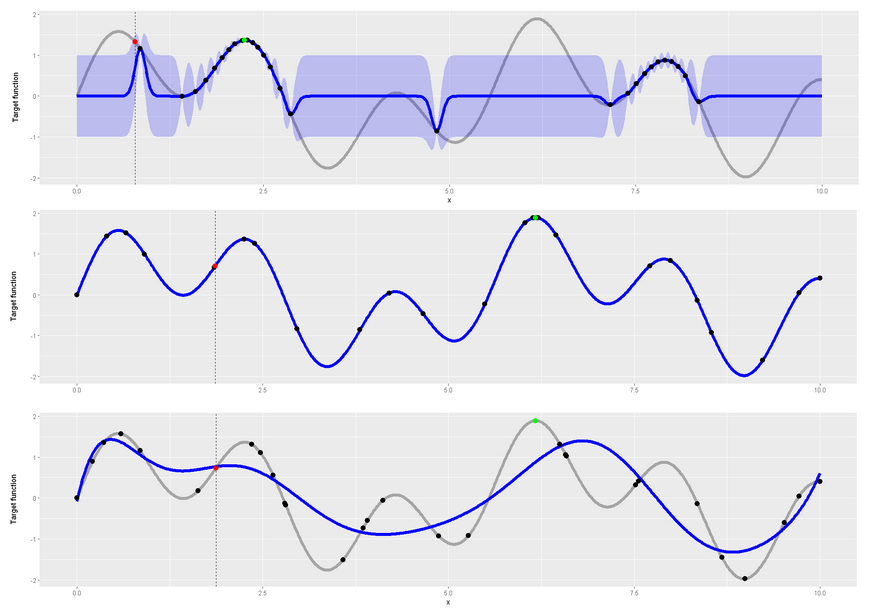
\includegraphics[width=\textwidth]{figures/bo_gp_kernel}
	\decoRule
	\caption[GP kernels]{Three GP regressions with different kernels $K(x,x')$ over the same target function: $e^{-100(x-x')^2}$ (top), $e^{-(x-x')^2}$ (middle) and $e^{-0.1(x-x')^2}$ (bottom). In the top plot each point has small influence over the rest, sampling new points inefficiently and resembling other local optimization techniques. In the bottom plot each point has too much small influence over the rest making a good fit impossible if the data varies more than expected. In the middle plot we can see a good fit with an appropriate kernel for the target function.}
	\label{fig:bo_gp_kernel}
\end{figure}

\begin{itemize}
\item \url{https://www.cs.toronto.edu/~duvenaud/cookbook/}
\item \url{https://nipunbatra.github.io/blog/ml/2021/09/03/param-learning-sgd.html}
\end{itemize}

\subsection{Batch iterations}
Each iteration we can select more than one candidate to evaluate. In expensive target functions this might be prohibitive, but in our case we might benefit for adding more information to the model. The batch size can be a modulation parameter depending on the computational cost of the function.

In the case of batches of more than one, we have to consider how those candidates are chosen: the maximum of the acquisition function is one, but the rest should be chosen such that the information provided is significant and not redundant given the rest (e.g. not too close to each other) [\cite{nguyen_budgeted_2017}][\cite{gonzalez_batch_nodate}].

\subsection{Constraints}

We suggest the use of the Constrained Expected Improvement acquisition function to incorporate constraints in the BO method [\cite{gardner_bayesian_nodate}]. An example can be seen in figure \ref{fig:bo_gp_regression_constraints}.

\begin{figure}[h]
	\centering
	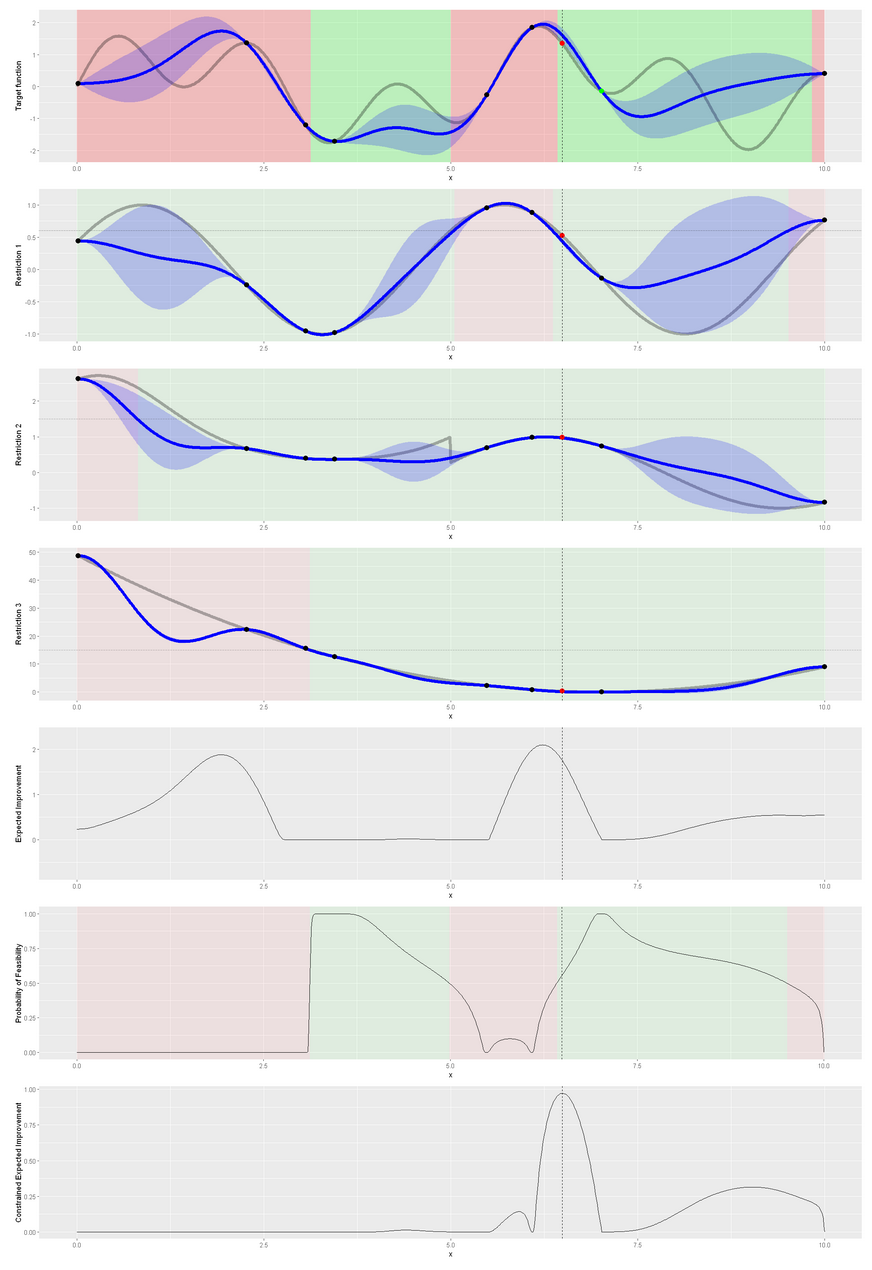
\includegraphics[width=\textwidth]{figures/bo_gp_regression_constraints}
	\decoRule
	\caption[Constrained Bayesian Optimization]{(Constrained) Bayesian Optimization using a Gaussian process after the eighth observed point. The acquisition function used is the Constrained Expected Improvement, combining the Expected Improvement with the probability of feasibility acquisition functions.}
	\label{fig:bo_gp_regression_constraints}
\end{figure}

Other alternative methods exist to incorporate constraints as well [\cite{paulson_cobalt_2021}][\cite{ungredda_bayesian_2021}][\cite{hernandez-lobato_general_2016}][\cite{swiler_survey_2020}][\cite{lam_lookahead_nodate}].

One related subject to constraints is the possibility to place priors on the input values to guide the optimization process [\cite{souza_bayesian_2021}]. Priors do not impose hard restrictions, only a starting hypothesis on the optimal values that gets progressively overshadowed in the presence of more evidence (i.e. data) [\cite{stark_constraints_2015}].

\section{Calibration over original inputs}

In the standard calibration procedure we change the transition probabilities in the matrices, assuming they are independent and enforcing constraints in the error calculation step. One alternative would be to calibrate over those relevant original inputs (i.e. those found in the literature, studies, expert opinions, ...) and then calculate the transition probabilities (and possibly other inputs of the model) from them. With this method we preserve and inject the knowledge we have about the domain into the model (that is, how to calculate the probabilities from the scientific sources, assumptions, implicit restrictions, ...).

\begin{figure}[h]
	\centering
	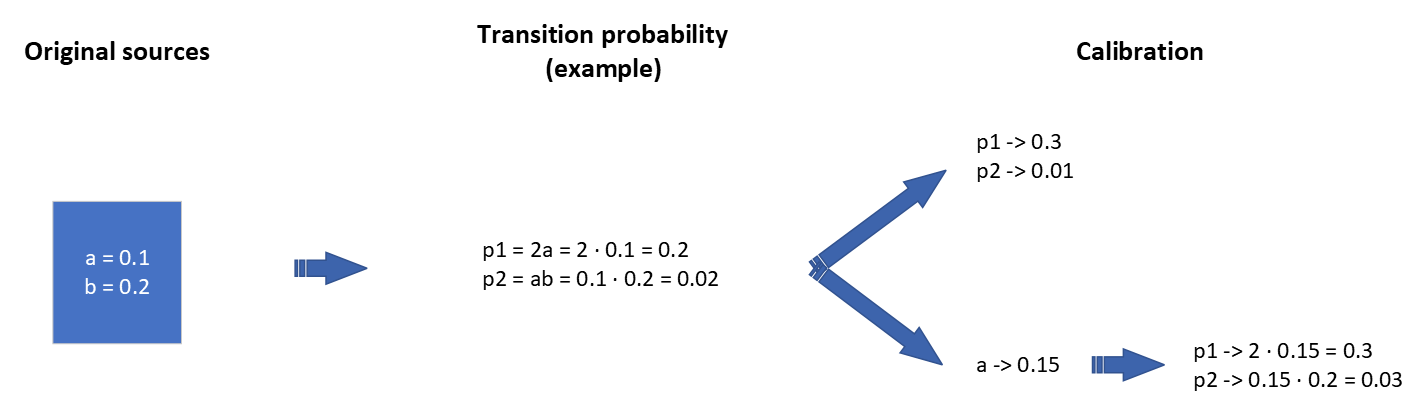
\includegraphics[width=\textwidth]{figures/calibration_inputs}
	\decoRule
	\caption[Calibration over inputs]{Calibration procedures: directly over the probabilities (``Calibration'', top) and over the original inputs (``Calibration'', bottom).}
	\label{fig:calibration_inputs}
\end{figure}

Since we calibrate to account for the uncertainty in the natural history and the probabilities in the matrices are calculated from parameters, we could classify the uncertainty sources in two: uncertainty associated to the inputs and uncertainty associated to the calculation of the probability.

\subsection{Parameter uncertainty}
If we are sure about the calculation of the transition probability, like a well-known relationship (e.g. Bayes formula), the remaining sources of uncertainty are the inputs themselves. In this case we can set up the optimizer to change these inputs, recalculate the probabilities and run the model.

For interpretation and sanity check purposes we can check both the changed input value and the newly-calculated transition probability.

\begin{figure}[h!]
	\centering
	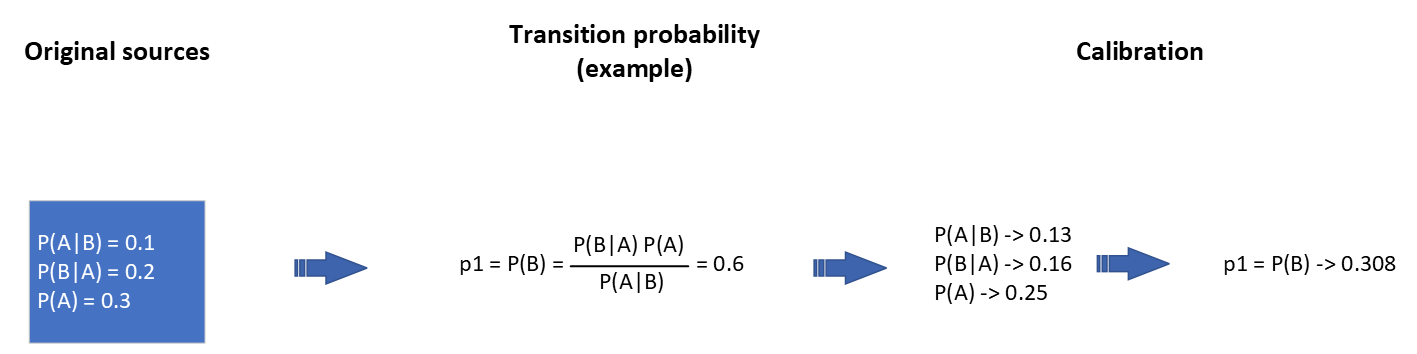
\includegraphics[width=\textwidth]{figures/calibration_values}
	\decoRule
	\caption[Calibration over input values]{If we are certain of the relationship between the probability and the inputs, we can calibrate over the inputs and we will get the calibrated probability by preserving the link with the original inputs.}
	\label{fig:calibration_values}
\end{figure}

\subsection{Calculation uncertainty}
Beyond the inputs, the calculation itself might be uncertain as well, for example by making a very rough approximation or assuming a probabilistic distribution with a poor fit. In this case we can insert an error term or scaling factor in the formula to account for the misspecification, with a neutral initial value (0 if error, 1 if factor). Then, the calibration could include these error/scaling terms in the set of parameters to be optimized.

For interpretation and sanity check purposes, besides the probabilities themselves as usual, we can check the error term/scaling factor. If they are too different from the initial values we might conclude that the calculation is not trustworthy and we might have to review our assumptions. Also, if the calculation is a very rough estimate another alternative would be to reject the calculation itself and optimize the probability value as usual.

\begin{figure}[h!]
	\centering
	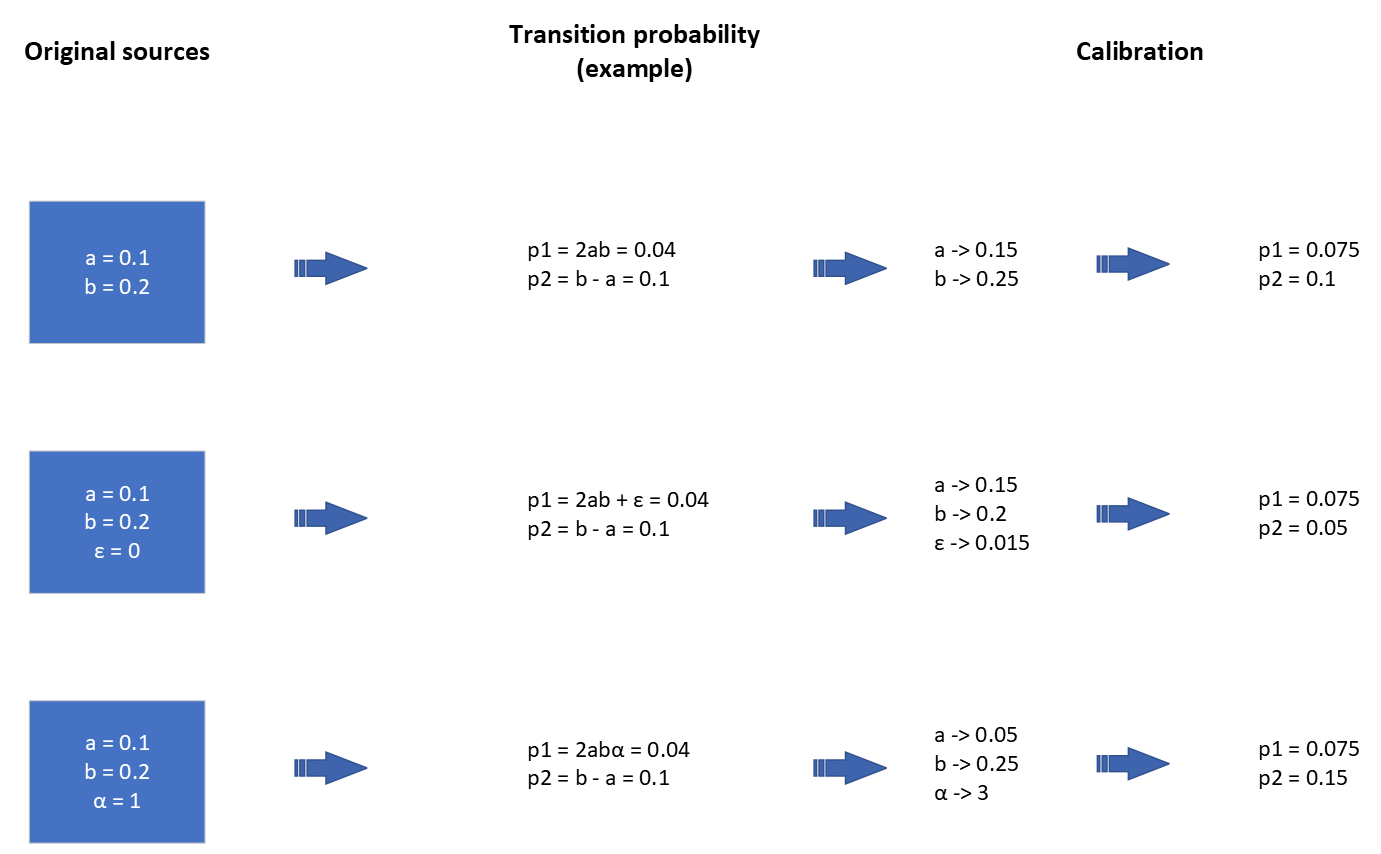
\includegraphics[width=\textwidth]{figures/calibration_calculation}
	\decoRule
	\caption[Calibration over calculations]{To account for the possibility of a misspecified calculation we can add additional terms to a formula. We can see calibration with no formula flexibility (top row), an additive error term for p1 (middle row) or a multiplicative factor for p1 (bottom row).}
	\label{fig:calibration_calculation}
\end{figure}

\subsection{Comments}

\subsubsection*{Pros}
\begin{itemize}
	\item Preserving the link and implicit knowledge between the original sources and the calculated probabilities
	\item Preserving relationships between probabilities and (some kinds of) constraints
\end{itemize}

\subsubsection*{Cons}
\begin{itemize}
	\item Overcomplicating the calibration procedure in simple cases
	\item Relationships might not be too complicated
\end{itemize}

\section{Input/probabilities dependencies using graph theory}

\begin{figure}[h!]
	\centering
	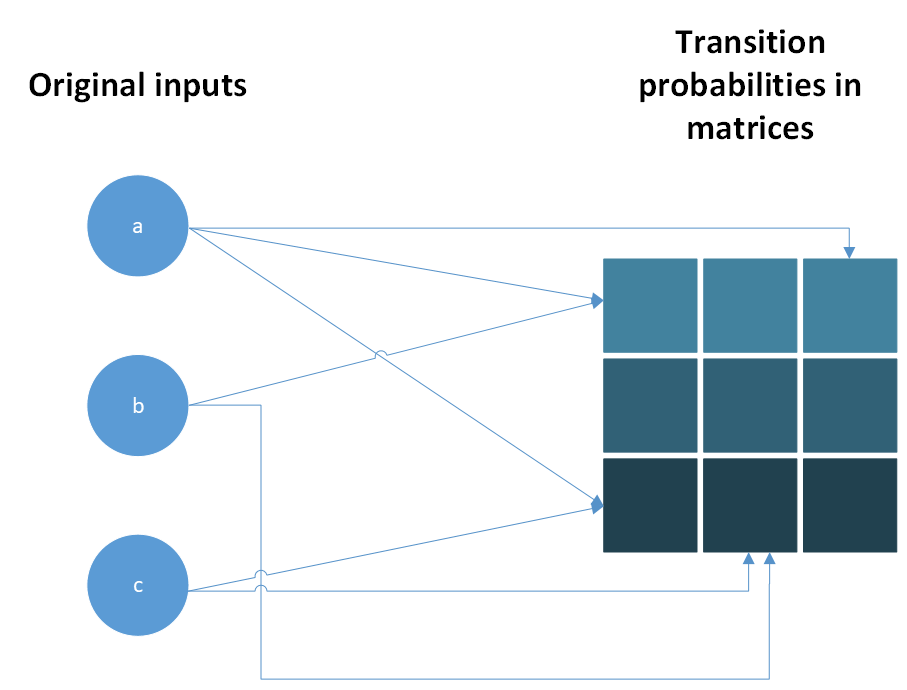
\includegraphics[width=\textwidth]{figures/graph_input_probs}
	\decoRule
	\caption[Dependency graph between inputs and transition probabilities]{We could use graph theory to help optimization considering the dependencies between inputs and the transition probabilities in the matrices.}
	\label{fig:graph_input_probs}
\end{figure}

\subsection{Comments}

\subsubsection*{Pros}
\begin{itemize}
	\item Might help the calibration procedure by exploiting domain knowledge
\end{itemize}

\subsubsection*{Cons}
\begin{itemize}
	\item Overcomplicating the calibration procedure in simple cases
	\item Relationships might not be too complicated
	\item Too vague at this point
\end{itemize}